\documentclass[journal=mamobx, layout=twocolumns,manuscript=article]{achemso}


\makeatletter

%%%%%%%%%%%%%%%%%%%%%%%%%%%%%% LyX specific LaTeX commands.


\title{Supporting information to the article\\ ``Water desalination using polyelectrolyte hydrogel. Gibbs ensemble modeling''}


\author{Mikhail Laktionov}

\affiliation[cuni]{Department of Physical and Macromolecular Chemistry, Faculty of Science,
Charles University in Prague, Czech Republic}


\alsoaffiliation[itmo]{St. Petersburg National Research University of Information Technologies,
Mechanics and Optics, St. Petersburg, Russia.}

\author{Lucie Nová}
\author{Oleg V. Rud}


\affiliation{Department of Physical and Macromolecular Chemistry, Faculty of Science,
Charles University in Prague, Czech Republic}


\alsoaffiliation[imc]{Institute of Macromolecular Compounds of Russian Academy of Sciences,
Saint-Petersburg, Russia}


\email{oleg.rud@natur.cuni.cz}



\abbreviations{MC, MD, RO, FO}


\keywords{polyelectrolye hydrogel, simulation, desalination}

%% Because html converters don't know tabularnewline
\providecommand{\tabularnewline}{\\}


%%%%%%%%%%%%%%%%%%%%%%%%%%%%%% User specified LaTeX commands.
%\usepackage[utf8]{inputenc}
\usepackage{amssymb}
%%%%%%%%%%%%%%%%%%%%%%%%%%%%%% User specified LaTeX commands.
\newcommand{\ie}{\textit{i.~e.} }
\newcommand{\cref}{c^{\ominus}}
%\newcommand{\cs}{c_{s}}
\newcommand{\kT}{k_\mathrm{B}T}
\newcommand{\kB}{k_\mathrm{B}}
\newcommand{\lb}{l_\mathrm{B}}
\newcommand{\NA}{N_{\mathrm{A^-}}}
\newcommand{\muna}{\mu_\mathrm{Na^+}}

\newcommand{\mucl}{\mu_\mathrm{Cl^-}}
\newcommand{\muca}{\mu_\mathrm{Ca^{2+}}}
\newcommand{\muh}{\mu_\mathrm{H^+}}
\newcommand{\mua}{\mu_\mathrm{A^-}}
\newcommand{\muha}{\mu_\mathrm{HA}}
\newcommand{\muoh}{\mu_\mathrm{OH}}

\newcommand{\cna}{c_\mathrm{Na^+}}
\newcommand{\ccl}{c_\mathrm{Cl^-}}
\newcommand{\cca}{c_\mathrm{Ca^{2+}}}
\newcommand{\ch}{c_\mathrm{H^+}}
\newcommand{\cp}{c_\mathrm{p}}
\newcommand{\nna}{n_\mathrm{Na^+}}
\newcommand{\ncl}{n_\mathrm{Cl^-}}
\newcommand{\Nna}{N_\mathrm{Na^+}}
\newcommand{\Ncl}{N_\mathrm{Cl^-}}

\newcommand{\ncleq}{\widetilde{N}_\mathrm{Cl^-}}
\newcommand{\nca}{N_\mathrm{Ca^{2+}}}

\newcommand{\superin}{^\mathrm{in}}
\newcommand{\subin}{_\mathrm{in}}
\newcommand{\subi}{_\mathrm{i}}

\newcommand{\gel}{^\mathrm{gel}}
\newcommand{\tot}{^\mathrm{tot}}
\newcommand{\out}{^{\mathrm{out}}}
\newcommand{\coh}{c_\mathrm{OH}}
\newcommand{\bulk}{^{\mathrm{b}}}
\renewcommand{\H}{\mathrm{H^+}}
\newcommand{\A}{\mathrm{A^-}}
\newcommand{\AH}{\mathrm{AH}}
%%%%%%%%%%%%%%%%%%%%%%%%%%%%%% LyX specific LaTeX commands.
%% A simple dot to overcome graphicx limitations
\newcommand{\lyxdot}{.}
\newcommand{\todoi}[1]{\todo[inline]{#1}}
\setuptodonotes{fancyline, color=blue!30, size=\tiny}

\newcommand{\cl}{\mathrm{Cl^-}}
\newcommand{\br}{\mathrm{Br^-}}
\newcommand{\na}{\mathrm{Na^+}}
\newcommand{\h}{\mathrm{H^+}}
\newcommand{\ka}{\mathrm{K^+}}
\newcommand{\oh}{\mathrm{OH^-}}
\newcommand{\ca}{\mathrm{Ca^{2+}}}
\newcommand{\mg}{\mathrm{Mg^{2+}}}
\newcommand{\so}{\mathrm{SO_4^{2-}}}

\newcommand{\EI}{E_{\mathrm{I}}}
\newcommand{\EII}{E_{\mathrm{II}}}
\newcommand{\SI}{S_{\mathrm{I}}}
\newcommand{\SII}{S_{\mathrm{II}}}
\newcommand{\NI}{N_{\mathrm{I}}}
\newcommand{\NII}{N_{\mathrm{II}}}
\newcommand{\VI}{V_{\mathrm{I}}}
\newcommand{\VII}{V_{\mathrm{II}}}
\newcommand{\FI}{F_{\mathrm{I}}}
\newcommand{\FII}{F_{\mathrm{II}}}
\newcommand{\nnaI}{N^{\na}_{\mathrm{I}}}
\newcommand{\nclI}{N^{\cl}_{\mathrm{I}}}
\newcommand{\nnaII}{N^{\na}_{\mathrm{II}}}
\newcommand{\nclII}{N^{\cl}_{\mathrm{II}}}




\newcommand{\Ka}{K_{\mathrm{A}}}
\newcommand{\pKa}{\mathrm{p}\Ka}
\newcommand{\pK}{\mathrm{p}K}
\newcommand{\pH}{\mathrm{pH}}
\newcommand{\mol}{\mathrm{mol}}
\newcommand{\molperl}{\mathrm{mol/l}}
\newcommand{\kg}{\mathrm{kg}}
\newcommand{\res}{^{\mathrm{res}}}
\newcommand{\pHres}{\pH\res}
\newcommand{\pHgel}{\pH\gel}
\newcommand{\cs}{c_{\mathrm{s}}}
%\newcommand{\cs}{c_{\mathrm{salt}}}
\newcommand{\csres}{\cs\res}
%\newcommand{\Vgel}{V\gel}
%\newcommand{\Vgel}{V_\mathrm{gel}}
\newcommand{\Vgel}{V}
\newcommand{\Ngel}{N_\mathrm{gel}}
%\newcommand{\Vgeleq}{\widetilde{V}_\mathrm{gel}}}
%\newcommand{\Pgel}{P_\mathrm{gel}}
\newcommand{\Pgel}{\Pi}
\newcommand{\Pres}{P_\mathrm{res}}
\newcommand{\Pout}{P_\mathrm{out}}
\newcommand{\Vout}{V_\mathrm{out}}
%\newcommand{\Vbox}{V_\mathrm{box}}
\newcommand{\Vbox}{V_0}
\newcommand{\PE}{polyelectrolyte{}}

\newcommand{\reffig}[1]{Figure~\ref{#1}}
\newcommand{\refeq}[1]{Equation~\ref{#1}{}}
\usepackage{afterpage}
\newcommand\blankpage{%
    \null
    \thispagestyle{empty}%
    \addtocounter{page}{-1}%
    \newpage}


\newcommand{\mytitle}{Gibbs ensemble for \PE{} hydrogel}
\newcommand{\etal}{\textit{et al.}{}}

\@ifundefined{showcaptionsetup}{}{%
 \PassOptionsToPackage{caption=false}{subfig}}
\usepackage{subfig}

\makeatother

\newpage

\begin{document}


\subsection{Ion exchange Monte Carlo sampling}
\paragraph{Open system.}
Consider the free energy in the grand-canonical ensemble for single particle type, \ie the Landau potential:
\begin{equation}
\Omega = E-TS + \mu N 
\end{equation}
where $E$ is internal energy, $T$~--- temperature, $S$~--- entropy, $N$ is the number of particles.
The entropy $S$ is given by the Boltzmann formula~\cite{Nagle2004}:
\begin{equation}
S= k_B \ln \frac{V^N}{N!}
\end{equation}
The change of free energy associated with insertion ($\xi=1$) or deletion ($\xi=-1$) a particle is
\begin{equation}
\Delta \Omega =\kT\ln\left(V^{\xi}\frac{N!}{ (N+\xi)!}\right)+\xi\mu+\Delta E
\end{equation}
In our case we insert ions only as electroneutral pairs, $\na$ and $\cl$, so the corresponding formula for the free energy change turns to 
\begin{equation}
\Delta\Omega=\kT\ln\left(V^{2\xi}\frac{\Nna!}{\left(\Nna+\xi\right)!}\frac{\Ncl!}{\left(\Ncl+\xi\right)!}\right)+
\xi\left(\muna+\mucl\right)+\Delta E
\label{eq: DeltaG RE one}
\end{equation}

In order to simulate an ensemble which exchanges particles with the bath (bulk reservoir) we need to perform the following Monte Carlo procedure \cite{Frenlkel2002_book}
\begin{enumerate}
	\item we propose the new configuration of the system by insertion (or deletion) of an ion pair so that the total number of pairs changes from $N$ to $N+\xi$, $\xi=\pm1$
	\item we accept the new configuration if $\mathcal{R}^{\xi}<e^{\Delta\Omega/\kT}$, where $\mathcal{R}$ is uniformly distributed random number in range between $0$ and $1$.
	\item continue untill the desired number of accepted moves is reached
\end{enumerate}





\paragraph{Closed system.}
In closed system ion pairs are exchanged between two finite volume boxes.
\begin{equation}
    \na_{I} + \cl_{I} \leftrightarrows \na_{II} + \cl_{II}
\end{equation}
Suppose an ion pair has been moved from one box to another, then the change in entropy can be expressed as
\begin{equation}
    \Delta S = 2 k_B \ln \left(\frac{V^{I}}{V^{II}} \right) ^ {\xi}  \left(\frac{(N_{Na^{+}}^{I}+\theta(\xi))(N_{Cl^{-}}^{I}+\theta(\xi))}{(N_{Na^{+}}^{II}+\theta(-\xi))(N_{Cl^{-}}^{II}+\theta(-\xi))}\right)^{-\xi}
\end{equation}
where $\xi$ again defines the direction of the trial move, so that $\xi_{I \rightarrow II} = -1$ when an ion pair moved from box I to box II and  $\xi_{II \rightarrow I} = 1$ otherwise, $\theta(\xi)$ is the Heaviside step function.
The corresponding total free energy change in both systems is the following 
\begin{equation}
\Delta\Omega = \Delta E^{I}+\Delta E^{II}+T\Delta S
\end{equation}
The Monte Carlo sampling procedure is the following
\begin{enumerate}
	\item propose the new configuration of the system by moving the ion pair from one volume to another 
	\item accept the new configuration if $\mathcal{R}^{\xi}<e^{\Delta\Omega/\kT}$
	\item continue untill the desired number of accepted moves is reached
\end{enumerate}

\subsection{Donnan equilibrium in finite volume reservoirs}
\todo{mb we remove this section}
Before we can explore any system properties and collect data the system has to be equilibrated. To achieve this we perform equilibration routine consist of sequence of Molecular Dynamics and Monte Carlo steps.
%Here we describe our technique
The result of equilibration is stationary of any observable such as pressure, end-to-end distance for polymer chains and ion distribution between reservoirs. 

The success and the cost in terms of computational time for the equilibration process heavily depend on initial guess. In our case we initialize the system with ion distribution corresponds to Donnan equilibrium.

In closed system number of ions in the system is constant, so Donnan equilibrium can be formulated as follows
\begin{equation}
    \frac{\left(N_{pairs} - N_{Cl^{-}}^{(gel)}\right)^2}{V_{salt}^2} = \frac{N_{Cl^{-}}^{gel} (N^{{(gel)}}_{A^{-}} + N_{Cl^{-}}^{(gel)})}{V_{gel}^2}
\end{equation}
where $N^{{(gel)}}_{A^{-}}$ is number of fixed anions in the box with the gel \ie acetic groups in the polymer gel.
Solving this equation with respect to $N^{{(gel)}}_{A^{-}}$ gives us the distribution of the ions between two boxes.


\begin{equation}
N_{Cl^{-}}^{(gel)} = \frac{\frac{\NA \Vout^{2}}{2} + N_{pairs} \Vgel^{2} - \frac{\Vout \sqrt{N^{{(gel)}}_{A^{-}}^{2} \Vout^{2} + 4 N^{{(gel)}}_{A^{-}} N_{pairs} \Vgel^{2} + 4 N_{pairs}^{2} \Vgel^{2}}}{2}}{\Vgel^{2} - \Vout^{2}}
\end{equation}

\todoi{
This paragraph moved from overleaf

Compression of the gel in infinite reservoir does not  change its salinity, on the contrary, upon compression of the gel in closed reservoir salinity of separated liquid is decreasing (supernatant salinity), using the Donnan law formulated for finite reservoir salinity can be expressed as
\begin{equation*}
    c_s^\prime = \frac{\sqrt{4\alpha^{2} c_{p}^{2} \left(1-\gamma\right)^{2} + \alpha c_{p} c_{s} \gamma^{2} + c_{s}^{2} \gamma^{2}}-\frac{\alpha c_{p} \left(1-\gamma\right)}{2} - c_{s} \left(1-\gamma\right)}{\gamma^{2} - \left(1-\gamma\right)^{2}}
\end{equation*}
where $\gamma = V_{gel}/V_0$ is relative to initial volume compression.
}
\begin{eqnarray}
    %N_{Cl^{-}}^{(gel)} = \frac{\frac{N^{{(gel)}}_{A^{-}} V_{salt}^{2}}{2} + N_{pairs} V_{gel}^{2} - \frac{V_{salt} \sqrt{N^{{(gel)}}_{A^{-}}^{2} V_{salt}^{2} + 4 N^{{(gel)}}_{A^{-}} N_{pairs} V_{gel}^{2} + 4 N_{pairs}^{2} V_{gel}^{2}}}{2}}{V_{gel}^{2} - V_{salt}^{2}}
    \\
    N_{Na^{+}}^{(gel)} = N^{{(gel)}}_{A^{-}} + N_{Cl^{-}}^{(gel)}
    \\
    N_{Cl^{-}}^{(salt)} = N_{Na^{+}}^{(gel)} = N_{pairs} - N_{Cl^{-}}^{(gel)}
\end{eqnarray}
\subsection{Sampling routine}
Data gained from Molecular Dynamics (MD) and Monte Carlo processes (MC) are highly autocorrelated, thus we can not imply statistic developed for uncorrelated data. 
We have written a small in-house python package realizing the routine estimating mean and error for the observables provided by simulation, \ie pressure, number of particles, end-to-end distance of a chain for a given confidence level or effective sample size. 
Within this routine we provided the way to limit sampling procedure with some timeout value, in a way similar to described in \href{https://www.physik.uni-leipzig.de/~janke/Paper/nic10_423_2002.pdf}{Janke2002}

The expected value of the observable $X$ is estimated as a simple sample mean of $\overline{X}$, just like for uncorrelated data. While estimating the errors and \emph{effective} sample size $N_{\text{eff}}$, the following formulas were used.
\begin{equation}
    N_{eff} = \frac{N}{2\tau}
\end{equation}    
\begin{equation}
    \tau  = \frac{1}{2} + \sum_{k=1}^{N} \text{acf} (k) (1-\frac{k}{N})
\end{equation}
where $\tau$ is integrated autocorrelation time, $N$ size of autocorrelated data, $\text{acf} (k)$ is autocorrelation function on lag.

Note that ideally integral of  $\text{acf} (k)$ monotonically approaches some finite value, but due to unavoidable errors in number representation in computer and numeric integration methods it does not hold. 
For that reason instead of $\text{acf} (k)$ integral we use the maximum of its cumulative sum.

Margins of error (MOE) for a given confidence level $\gamma$ and effective sample size $N_{eff}$ is calculated using the following equation:
\begin{eqnarray}
    \text{MOE}(\gamma) = \frac{S_{N}}{\sqrt{N_{\text{eff}}}} t_{((1+\gamma)/2, N_{\text{eff}}-1)}
\end{eqnarray}
where $t_{(\alpha, \nu)}$ is percentile function (inverse cumulative distribution function) of Student’s distribution with $\nu$ degrees of freedom for $\alpha$ percentile,
$S_N$ is standard deviation of the sample.
The true mean of the observable $\mu_X$ lies inside the confidence interval with the confidence level $\gamma$.
\begin{equation}
    \Pr(\overline{X} - MOE(\gamma) \leq \mu_X \leq \overline{X} + MOE(\gamma)) = \gamma
\end{equation}
In our study we set $\gamma = 0.95$


\paragraph{Routine implementation details.}
%Probably we don't need this section

The sampling routine takes the function calculating an observable $X$ as an argument. 
In addition, it takes as a parameter one of the following values: the desired margins of error, target effective sample size or timeout.
An observable is sampled in a loop till one of required targets is met (timeout, the margins of error or sample size). 
In the each following iteration of the loop, mean value and the margins of error are calculated with ever increasing precision and sample size. 

The loop follows the next steps:
\begin{itemize}
    \item Sample new data to double the sample size
    \item Recalculate $\tau$, $N_{eff}$, and MOE
    \item Exit the loop if either MOE is less than the desired, 
    			or $N_{eff}$ is bigger than the desired, 
    			or run time exceed timeout.
\end{itemize}
Finally, it returns mean of the sample, margins of error that defines confidence interval where true mean of distribution lies and \emph{effective} sample size. 
The routine is also described schematically in Figure \ref{fig: sampling_diagram}

\begin{figure*}[t]
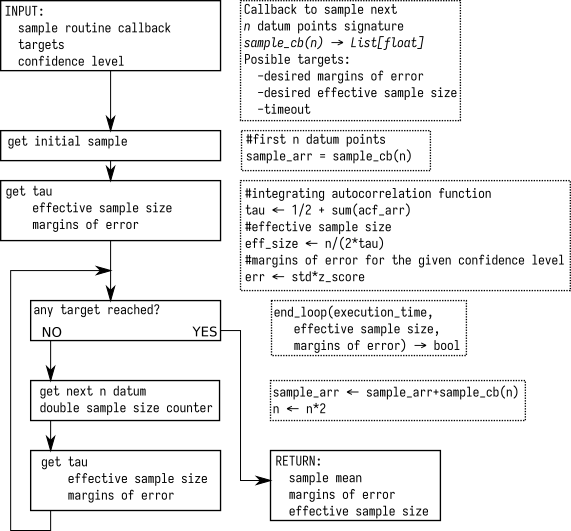
\includegraphics[width = 0.9\textwidth]{figures/sample_to_target_scheme.png}
\caption{Sampling routine diagram}
\label{fig: sampling_diagram}
\end{figure*}
\bibliographystyle{plain}
\bibliography{lit/gibbs.bib}
\end{document}